%----------------------------------------------------------------------------------------
%	PACKAGES AND DOCUMENT CONFIGURATIONS
%----------------------------------------------------------------------------------------
\documentclass[11pt]{article}
\usepackage{amsmath} % Required for some math elements
\usepackage{hyperref} 
\usepackage{xcolor}
\usepackage{lipsum} 
\usepackage{cite}
\usepackage{graphicx} % Required for the inclusion of images
\usepackage{algorithmic}
\usepackage{array}
\usepackage{bookmark}
\usepackage{listings}
\usepackage{amssymb}
\usepackage{enumitem}
\usepackage[margin=24mm]{geometry}
\usepackage[caption=false, font=footnotesize]{subfig}
\usepackage{multirow}
\usepackage[active,tightpage]{preview}

\renewcommand{\PreviewBorder}{1in}
\newcommand{\Newpage}{\end{preview}\begin{preview}}

\newlist{steps}{enumerate}{1}
\setlist[steps, 1]{label = Step \arabic*:}

\hypersetup{ %color attributes of citation, link, etc.
    colorlinks=true,
    linkcolor=blue,
    filecolor=gray,      
    urlcolor=blue,
    citecolor=blue,
}


\definecolor{mGreen}{rgb}{0,0.6,0}
\definecolor{mGray}{rgb}{0.5,0.5,0.5}
\definecolor{mPurple}{rgb}{0.58,0,0.82}
\definecolor{backgroundColour}{rgb}{0.95,0.95,0.92}

\lstdefinestyle{Cstyle}{
    backgroundcolor=\color{backgroundColour},   
    commentstyle=\color{mGreen},
    keywordstyle=\color{magenta},
    numberstyle=\tiny\color{mGray},
    stringstyle=\color{mPurple},
    basicstyle=\footnotesize,
    breakatwhitespace=false,         
    breaklines=true,                 
    captionpos=b,                    
    keepspaces=true,                 
    numbers=left,                    
    numbersep=5pt,                  
    showspaces=false,                
    showstringspaces=false,
    showtabs=false,                  
    tabsize=2,
    language=C
}


\newcommand{\matlab}{\textsc{Matlab }} %very important and totally necessary addition

\newcommand\Item[1][]{%
  \ifx\relax#1\relax  \item \else \item[#1] \fi
  \abovedisplayskip=0pt\abovedisplayshortskip=0pt~\vspace*{-\baselineskip}}
  %----------------------------------------------------------------------------------------
%	DOCUMENT INFORMATION
%----------------------------------------------------------------------------------------
 
\title{ECEN301 : Embedded Systems \\ Lab 2 Submission}
\author{Daniel Eisen : 300447549}
\date{\today}

\begin{document}
\begin{preview}
\maketitle
%----------------------------------------------------------------------------------------
%	DOCUMENT CONTENT
%----------------------------------------------------------------------------------------
\section{Objectives}
This lab demonstrated the use of the analogue to digital convertor onboard the 8051 as well as displaying data to a discrete LCD display. Using that as a base we covered analogue sensor input (in the form of a thermistor) as well as calibration, linearization and unit conversion. Side effects of this was encountering the limitations that an embedded engineer must overcome, such as small stack size, peripheral type limitations etc.     

\section{Methodology}
        \subsection{Introduction}
        This lab requires the 8051, the LCD display (control to P4, data to P0), and breadboard module with a variable voltage divider module attached. As with the last lab, the programs were developed and compiled to a hex file with Atmel Studio and the included 8051 library and lab modules library.
        
        Initially LCD control was tested with basic IO, then familiarising ourselves with the ADC by designing a basic voltmeter, then finally, with more complexity a temperature measurement program was designed and calibrated.   

        \subsection{LCD Display}
        \begin{center}
                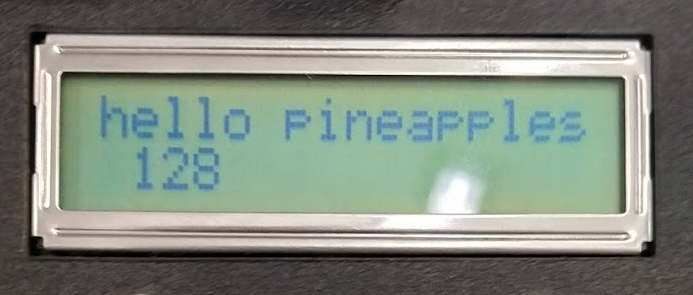
\includegraphics[width=0.65\textwidth]{res/LCD0.jpg}

                \textit{Fig. 1 LCD text and number}
        \end{center}

        Connecting the module as outline above to the 8051
        
        \lstinputlisting[language=C,style=CStyle]{res/lcd.c}

        \subsection{ADC}
        \begin{center}
                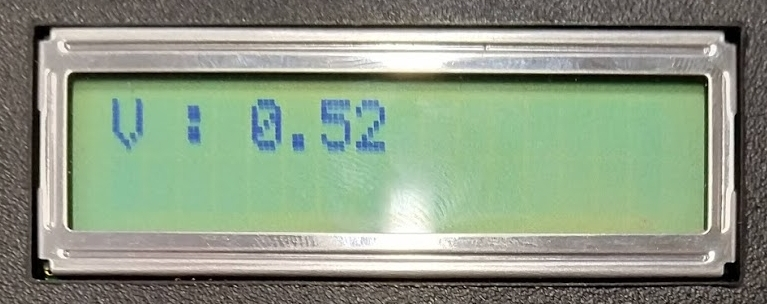
\includegraphics[width=0.45\textwidth]{res/vmeasure0.jpg}
                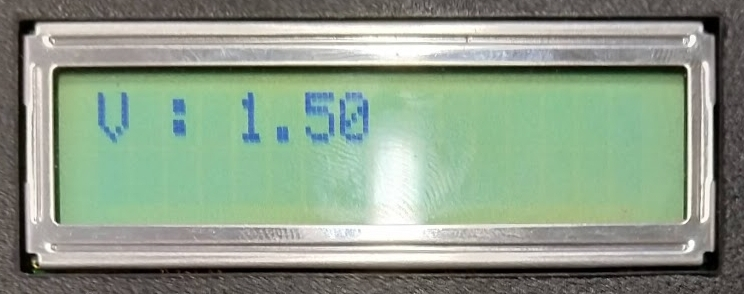
\includegraphics[width=0.45\textwidth]{res/vmeasure1.jpg}
                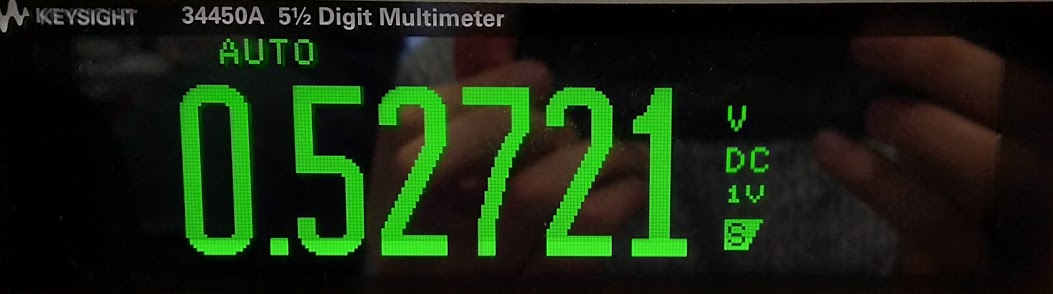
\includegraphics[width=0.45\textwidth]{res/vactual0.jpg}
                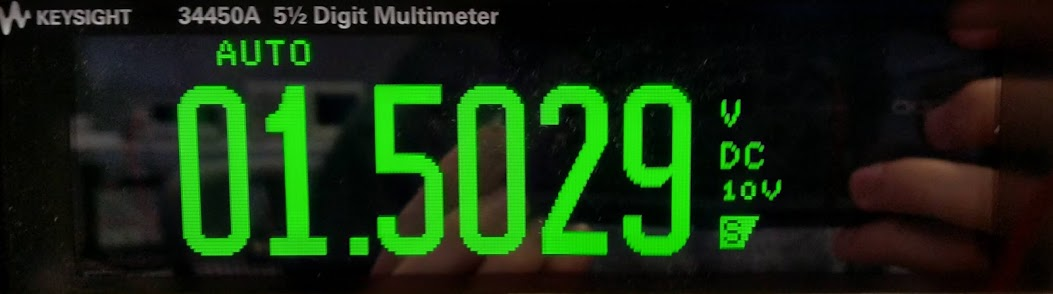
\includegraphics[width=0.45\textwidth]{res/vactual1.jpg}
        \end{center}

        \lstinputlisting[language=C,style=CStyle]{res/volt.c}

        \subsection{Temperature}
        \lstinputlisting[language=C,style=CStyle]{res/temp.c}
\section{Questions}
\begin{enumerate}
        \item \textit{Explain what all of the bits in the ADCON and ADCF registers mean?} \\
        \begin{itemize}
                \item ADCF is the 'ADC Configuration' register. Setting one of the bits in this register enable the corresponding pin on Port 1 for the input to the ADC, (Clearing sets it back to standard IO).
                \item ADCON is the control register for the ADC:
                \begin{itemize}
                        \item Bit 7 is reserved
                        \item Bit 6, set this to enable "pseudo idle mode." Basically putting the cpu into sort of sleep/low actively mode that allow the full 10bits of data from ADC to be used. This is due to the reduction in cpu noise.
                        \item Bit 5 enables/standbys the ADC. If code doesn't use the adc clearing this can save power.
                        \item Bit 4 is a flag that is set when the adc and finished doing a reading, this needs to be cleared by your code.
                        \item Bit 3 is used to start the conversion, this cleared afterward by the hardware.
                        \item Bit 2:0 are used to select between the 8 input channels
                \end{itemize} 
        \end{itemize}

\end{enumerate}

\end{preview}
\end{document}